\chapter{Маршевый метод коротких характеристик}

\section{Численные методы для стационарных гиперболических задач}

Уравнение переноса излучения относится к классу стационарных гиперболических уравнений. Стационарное гиперболическое уравнение должно содержать времениподобную переменную. Например, для задачи сверхзвукового обтекания такой переменной может быть выбрано направление, в котором поток газа или жидкости движется со сверхзвуковой скоростью. Для задачи переноса излучения времениподобной переменной является координата $s$ вдоль направления излучения $\vec \Omega$. 

Для гиперболических уравнений разработан ряд методов, например, сеточно-характеристические методы \cite{magometov1988}, различные TVD методы \cite{Godunov1959,vanLeer1974,Leveque2002,Toro2009}, ENO и WENO схемы \cite{Shu1998} и разрывный метод Галеркина \cite{Cockburn1989}. Для применения этих методов к уравнению переноса следует сначала дискретизировать угловую часть функции интенсивности $I(\vec r, \vec \Omega) \to I_i(\vec r)$. Для этой задачи имеется два основных подхода:
\begin{itemize}
\item дискретизация на некоторой сетке направлений $\vec \omega_i$, при этом $I_i(\vec r) = I(\vec r, \vec \omega_i)$;
\item дискретизация усреднением.
\end{itemize}
В последнем случае сфера направлений разбивается на участки $\Sigma_i$, например, триангулируется. Далее, уравнение переноса 
\[
(\vec \Omega \nabla) I(\vec r, \vec \Omega) + \varkappa(\vec r, \vec \Omega) I(\vec r, \vec \Omega) = \varkappa(\vec r, \vec \Omega) I_\text{p}(\vec r, \vec \Omega),
\]
которое можно записать в дивергентном виде
\[
\div \left(\vec \Omega I(\vec r, \vec \Omega)\right) + \varkappa(\vec r, \vec \Omega) I(\vec r, \vec \Omega) = \varkappa(\vec r, \vec \Omega) I_\text{p}(\vec r, \vec \Omega),
\]
усредняется по каждому участку $\vec \Omega \in \Sigma_i$. При этом
\[
I_i(\vec r) = \int\limits_{\Sigma_i} I(\vec r, \vec \Omega) d\Omega,
\]
а при усреднении $\vec \Omega I(\vec r, \vec \Omega)$ обычно предполагается зависимость среднего только от $I_i(\vec r)$:
\[
\int\limits_{\Sigma_i} \vec \Omega I(\vec r, \vec \Omega) d\Omega \sim I_i(\vec r).
\]
Если обозначить
\[
\vec \omega_i \equiv \frac{\int_{\Sigma_i} \vec \Omega I(\vec r, \vec \Omega) d\Omega}{\int_{\Sigma_i} I(\vec r, \vec \Omega) d\Omega},
\]
усредненное уравнение переноса принимает простой вид, аналогичный уравнению, дискретизированному на сетке направлений $\vec \omega_i$
\begin{equation}
\div (\vec \omega_i I_i(\vec r)) + \varkappa_i(\vec r) I_i(\vec r) = \varkappa_i(\vec r) I_{\text{p},i}(\vec r),\quad i = 1, \dots, K.
\label{eq:grid}
\end{equation}

Вне зависимости от способа получения, система \eqref{eq:grid} является системой независимых уравнений переноса в направлениях $\vec \omega_i$, и может быть решена вдоль всех направлений параллельно. Необходимо отметить, что метод, построенный на основании системы \eqref{eq:grid}, всегда будет испытывать <<эффект луча>>, так как излучение от источника может распространяться только в направлениях $\vec \omega_i$ и ни в каких других.



Рассмотрим отдельно $i$-е уравнение. Характеристикой данного уравнения является луч $\vec r - \vec r_0 = \vec \omega_i s$. 
Для уравнения переноса сеточно-характеристический метод называется методом коротких характеристик В метода коротких характеристик лежит идея интерполяции сеточных величин в основании характеристики $I_i^*$ и дальнейшего интегрирования решения уравнения вдоль характеристики (см. рисунок \ref{fig:char}). При этом найти решение в точке $\vec r_p$, из которой выпущена характеристика возможно лишь после того, как во всех узлах грани, содержащей основание характеристики, решение уже найдено. Будем далее назвать грань \emph{освещенной}, если интенсивность излучения $I_i$ во всех узлах на ней известна.
\begin{figure}[ht!]
\centering
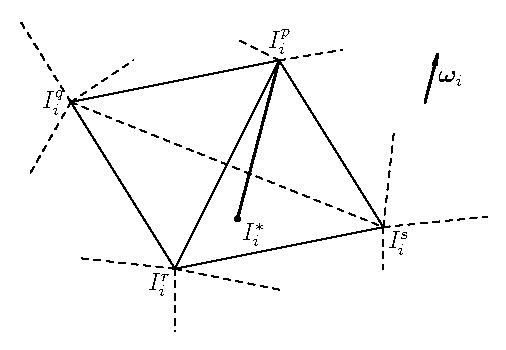
\includegraphics[height=.3\textheight]{radiation-2.eps}
\caption{Схема сеточно-характеристического метода}
\label{fig:char}
\end{figure}

Простейшим представителем конечно-объёмных методов является метод Годунова. В основе конечно-объемных методов лежат интегральные законы сохранения. Проинтегрируем уравнение переноса
\eqref{eq:grid} по объему тетраэдра $T$ (для краткости будем опускать индекс направления $i$):
\[
\int\limits_T \div (\vec \omega I(\vec r))  d\vec r + \int\limits_T \varkappa(\vec r) I(\vec r)  d\vec r = \int\limits_T \varkappa(\vec r) I_\text{p}(\vec r)  d\vec r.
\]
Интеграл от дивергенции может быть записан в виде интеграла по границе:
\[
\int\limits_T \div (\vec \omega I(\vec r)) d\vec r= \int_{\partial T} \vec n \vec \omega I(\vec r) d\Gamma.
\]
В конечно-объемных методах нормальный поток на границе конечного объема определяется из точного либо приближенного решения задачи Римана о распаде разрыва \cite{Kulikovskiy2001}.
Для уравнения переноса излучения задача Римана имеет простое решение. Пусть значение интенсивности излучения в полупространстве $\vec r \vec n < 0$ равно $I_L$, а значение в полупространстве $\vec r \vec n > 0$ равно $I_R$. Тогда поток интенсивности излучения $\vec \omega I$ через границу $\vec r \vec n = 0$ равен
\[
\vec \omega I\big|_{\vec r \vec n = 0} = 
\begin{cases}
\vec \omega I_L, &\vec \omega \vec n > 0\\
\vec \omega I_R, &\vec \omega \vec n \leq 0
\end{cases}.
\] 
Заметим, что отнесение $\vec \omega \vec n = 0$ к одному из этих случаев несущественно, так как нормальный поток в любом случае будет равен нулю.

Назовем грань $f_j$ тетраэдра $T$ \emph{входной}, если внешняя нормаль $\vec n_j$ составляет с направлением изучения $\vec \omega$ тупой угол, и \emph{выходной} в противном случае.
Примем гипотезу о постоянном распределении величин $I, \varkappa, I_{\text{p}}$ в тетраэдре $T$. Обозначим $I^0$ интенсивность излучения в тетраэдре $T$, а $I^j$ --- интенсивность излучения в тетраэдре, граничащем с $T$ по грани $f_j$. Используя выражение для нормального потока из решения задачи Римана, получаем метод Годунова для уравнения переноса излучения:
\begin{equation}
\frac{1}{V(T)}\left[
\sum_{\substack{f_j \in \partial T\\\vec n_j \vec \omega < 0}} \vec S_j \vec \omega I^j 
+
\sum_{\substack{f_j \in \partial T\\\vec n_j \vec \omega > 0}} \vec S_j \vec \omega I^0
\right]
+ \varkappa I^0 = \varkappa I_\text{p},
\label{eq:fvm}
\end{equation}
где посредством $\vec S_j$обозначена векторная площадь грани $j$, то есть площадь, умноженная на внешнюю нормаль $\vec n_j$, а $V(T)$ --- объём тетраэдра $T$. Можно видеть, что для определения $I^0$ необходимо знать интенсивность излучения $I^j$ во всех тетраэдрах, граничащих с $T$ по его входным граням.

Разностные задачи, полученные либо сеточно-характеристичекими, либо конечно-объёмными методами, представляют собой набор линейных уравнений относительно неизвестных значений интенсивности. Данные уравнения можно решить итерационно, например методом установления, фактически превратив исходную стационарную гиперболическую задачу в нестационарную. Однако, эти задачи могут быть решены и безытерационным методами, в которых решение строится последовательным обходом неизвестных (маршем), при котором для вычисления очередной неизвестной все необходимые данные были найдены раньше.
Данные методы имеют преимущество, так как требуют лишь однократного прохода по расчетной области, в отличие от итерационных методов, в которых необходимо многократно повторять вычисления для каждого узла до достижения требуемой точности.

\section{Метод коротких характеристик второго порядка аппроксимации}

Рассмотрим метод коротких характеристик, в котором интенсивность излучения задана в нескольких узлах на гранях тетраэдров, но без конкретизации расположения данных узлов и их количества. Будем предполагать, что коэффициенты поглощения и интенсивность равновесного излучения постоянны в каждом тетраэдре.

Для определения решения на грани требуется определить решение в каждом узле, расположенном на данной грани. Для этого из каждого узла грани выпускается характеристика в направлении $-\vec\omega$ до пересечения с гранью тетраэдра (см. рисунок \ref{fig:manychar}). Заметим, что эта грань будет входной, так как характеристика выходит из тетраэдра в направлении $-\vec\omega$ под острым углом к нормали $\vec n$ к грани. Различные характеристики могут выходить из тетраэдра через различные входные грани, поэтому до вычисления решения на выходной грани, все входные грани должны быть уже освещены (то есть, решение на них уже должно быть найдено).
\begin{figure}[ht!]
\centering
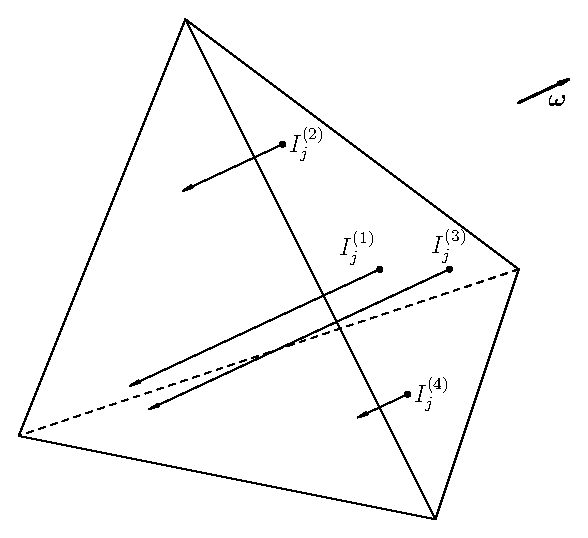
\includegraphics[height=.3\textheight]{radiation-4.eps}
\caption{Характеристики, выпущенные из нескольких узлов на грани тетраэдра}
\label{fig:manychar}
\end{figure}

Вдоль каждой характеристики уравнение переноса является обыкновенным дифференциальным уравнением
\[
\frac{dI}{ds} + \varkappa I = \varkappa I_\text{p},
\]
причем величины $\varkappa$ и $I_\text{p}$ постоянны по предположению. Решение этого уравнения может быть записано в виде
\begin{equation}
I = e^{-\tau} I^*  + \left(1 - e^{-\tau}\right) I_\text{p},
\label{eq:shortchar}
\end{equation}
где $I$ --- интенсивность излучения в точке, из которой выпускается характеристика, $I^*$ --- интенсивность излучения в точке пересечения характеристики с входной гранью, а $\tau$ --- оптическая длина характеристики, равная ее длине $\ell$, умноженной на коэффициент поглощения $\varkappa$. Из \eqref{eq:shortchar} следует, что интенсивность $I$ не выходит за диапазон значений $[\min(I^*, I_\text{p}), \max(I^*, I_\text{p})]$.

Величина $I^*$ определяется интерполяцией по значениям интенсивности в узлах той грани, через которую выходит характеристика. Порядок аппроксимации метода соответствует степени используемой интерполяции. Для получения метода второго порядка необходимо пользоваться квадратичной интерполяцией значений интенсивности на грани, при этом необходимо знать значение интенсивности в шести узлах на данной грани.

Повысить порядок метода можно и не увеличивая количество узлов на грани, а пользуясь значениями интенсивности на соседних гранях. Однако, данный способ увеличивает разностный шаблон, нарушая компактность схемы. При расширении шаблона появляются дополнительные зависимости между решением на различных гранях, что существенно осложняет алгоритм упорядочения неизвестных.

Таким образом, для построения метода второго порядка необходимо на каждой грани выбрать шесть узлов интерполяции.

\subsection{Расположение узловых точек}

Расположение узлов интерполяции на грани не может быть произвольным. Применим данный метод к двумерному уравнению переноса излучения на равномерной прямоугольной сетке. Ограничимся методом первого порядка. На каждой грани (которая в двумерном случае является просто отрезком) возьмем два узла для линейной интерполяции, но расположим их строго внутри грани (см. рисунок \ref{fig:instab}).

В случае, когда излучение распространяется под малым углом к вертикали $\omega_x < \sin \theta_\text{кр}$, численное решение переносится только вертикально, при этом нарушается необходимое условие устойчивости разностного метода: область зависимости численного решения не содержит область зависимости решения дифференциальной задачи. Пусть $I_j^{(1)}$ и $I_j^{(2)}$ --- значения интенсивности соответственно в левом и правом узле на $j$-ом слое в некотором фиксированном столбце. Тогда в простейшем случае $\varkappa = 0, I_\text{p} = 0$ численное решение удовлетворяет соотношениям
\begin{gather*}
I_{j+1}^{(1)} = I_{j}^{(1)} - \frac{\omega_x}{\omega_y} \frac{I_{j}^{(2)} - I_{j}^{(1)}}{1 - 2\tg \theta_\text{кр}},\\
I_{j+1}^{(2)} = I_{j}^{(2)} - \frac{\omega_x}{\omega_y} \frac{I_{j}^{(2)} - I_{j}^{(1)}}{1 - 2\tg \theta_\text{кр}}.
\end{gather*}
В зависимости от знака $I_0^{(2)} - I_0^{(1)}$ решение $I_j^{(1,2)}$ неограниченно стремится либо к $+\infty$, либо к $-\infty$.

\begin{figure}[ht!]
\centering
\includegraphics[height=.4\textheight]{instab-0.eps}
\caption{Направление распространения излучения в численной схеме (контурная стрелка) и истинное направление $\vec \omega$}
\label{fig:instab}
\end{figure}

Данный эффект не возможен, если узлы располагать в вершинах сетки. При этом $\theta_\text{кр} = 0$. По данной причине в методе второго порядка узлы на гранях обязательно должны содержать 
вершины грани. Расположение остальных трех узлов может быть произвольно, но для простоты эти узлы были взяты на ребрах грани.

\subsection{Монотонизация схемы}

Как известно из теоремы Годунова, никакая линейная схема выше первого порядка не может быть монотонной. Немонотонность схемы второго порядка может приводить к нарушению выполнения принципа максимума, а также появлению нефизических (отрицательных) значений интенсивности. Из \eqref{eq:shortchar} следует, что процедура интегрирования вдоль характеристики является монотонной, а немонотонность может быть вызвана только интерполяцией интенсивности по грани.

Рассмотрим треугольную грань $T$ и квадратичную форму $I(\vec \xi)$ на ней. Чтобы форма была монотонной на грани $T$ необходимо, чтобы на всех ребрах грани $T$ форма была монотонна.
Если $I_1$ и $I_2$ --- значения формы на концах ребра, а $I_\text{ц}$ --- значение формы в середине ребра, то квадратичная форма на ребре имеет вид
\[
I(t) = I_\text{ц} + \frac{I_2 - I_1}{2} t + \frac{I_1 -2 I_\text{ц} + I_2}{2} t^2,
\]
где $t$ --- координата вдоль ребра, принимающая в концах ребра значения $\pm 1$. Эта форма не будет иметь экстремумов на интервале $t \in (-1, 1)$ при выполнении условия
\[
\left|\frac{I_2 - I_1}{2}\right| \geq |I_1 -2 I_\text{ц} + I_2|,
\]
что также можно записать в виде
\begin{equation}
\left|I_\text{ц} - \frac{I_1 + I_2}{2}\right| \leq \frac{|I_2 - I_1|}{4}.
\label{eq:mono}
\end{equation}
При выполнении этого условия максимум и минимум квадратичной формы $I(\vec \xi)$ по границе $\partial T$ достигается в вершинах треугольника $T$. Таким образом, если квадратичная форма $I(\vec \xi)$ имеет на треугольнике $T$ значения, выходящие за пределы значений в вершинах, то это может произойти лишь строго внутри треугольника. Иными словами, внутри треугольника должен находиться экстремум квадратичной формы $I(\vec \xi)$. Но при этом некоторые линии уровня $I(\vec \xi) = 0$ будут касаться сторон треугольника (см. рисунок \ref{fig:extr}), что означает существование локального экстремума квадратичной формы на ребре. Но это невозможно, а следовательно, квадратичная форма не может иметь локальных экстремумов внутри треугольника и является в нем монотонной.
\begin{figure}[ht!]
\centering
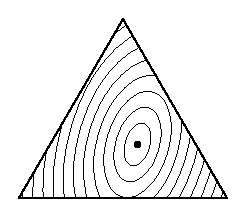
\includegraphics[height=.3\textheight]{extr-1.eps}
\caption{Линии уровня квадратичной формы при наличии экстремума внутри треугольника}
\label{fig:extr}
\end{figure}

Таким образом, условие монотонности \eqref{eq:mono} формы на ребрах является необходимым и достаточным для монотонности на всем треугольнике. Обеспечить его выполнение можно коррекцией значения в центре ребра $I_\text{ц}$:
\[
I_\text{ц}^\text{корр} = 
\frac{I_1 + I_2}{2} + \operatorname{clamp}\left(
I_\text{ц} - \frac{I_1 + I_2}{2}, 
\left[
-\frac{|I_2 - I_1|}{4},
\frac{|I_2 - I_1|}{4}
\right]
\right),
\]
где функция $\operatorname{clamp}(x, [a, b])$ <<зажимает>> значение $x$ в пределах отрезка $[a, b]$ и определяется как
\[
\operatorname{clamp}(x, [a, b]) = \max(a, \min(b, x)).
\]

Можно видеть, что метод второго порядка с данным ограничителем не хуже метода первого порядка, так как метод первого порядка получается при ограничении по правилу
\[
I_\text{ц}^\text{корр} = \frac{I_1 + I_2}{2}.
\]

\section{Алгоритмы упорядочения сеточных элементов}

Выше было показано, что как сеточно-характеристические, так и конечно-объемные схемы допускают построение численного решения маршевым образом. Для этого необходимо ввести порядок, в котором вычисляется решение по граням тетраэдров. Будем говорить, что тетраэдр $T$ следует за тетраэдром $T'$ ($T \succ T'$) если их общая грань является выходной для $T'$ и входной для $T$. В конечно-объемных методах решение в тетраэдре $T$ можно вычислить тогда, когда решения во всех предшествующих ему тетраэдрах $T' \prec T$ уже вычислены. В сеточно-характеристических методах вычисление решения в тетраэдре $T$ можно отождествить с вычислением решения на всех его выходных гранях, при этом необходимо знать решение на всех входных гранях, что соответствует нахождению решения во всех предшествующих ему тетраэдрах $T' \prec T$. Таким образом, упорядочение тетраэдров относительно отношения $T' \prec T$ является основой маршевого алгоритма как для сеточно-характеристических, так и для конечно-объемного методов.

Граф, связанный с отношением $\succ$, является ориентированным. Назовем упорядочением графа такую нумерацию тетраэдров $c(T)$ такую, что \[c(T) < c(T') \Leftrightarrow T \prec T'.\]
Нумерация не обязана быть инъективной, то есть из $c(T) = c(T')$ не обязано следовать, что $T = T'$.
Очевидно, что если в графе есть цикл
\[
T \prec T' \prec \dots \prec T'' \prec T,
\]
то упорядочение невозможно в силу $c(T) < \dots < c(T)$. Будем предполагать, что граф, связанный с отношением $\succ$ является направленным ациклическим графом. Известно \cite{Kahn1962}, что направленный ациклический граф всегда можно упорядочить.

\subsection{Алгоритм для триангуляций Делоне}

Предположим, что триангуляция области удовлетворяет условию Делоне, то есть для каждого тетраэдра $T$ в его описанной сфере не содержится целиком никакой другой тетраэдр $T'$.
Пусть $\pi(T) = \vec \omega \vec r_c(T)$, где $\vec r_c(T)$ --- радиус вектор центра описанной вокруг $T$ сферы, $\vec \omega$ --- направление излучения. Тогда сортировка тетраэдров по возрастанию значения $\pi(T)$ дает необходимый порядок $c(T)$, то есть $T \prec T' \Rightarrow \pi(T) < \pi(T')$ \cite{skalko2014}.

Докажем данное утверждение. Предположим, что для некоторой пары $T \succ T'$ выполняется $\pi(T) < \pi(T')$. Пусть $O, O'$ --- центры описанных вокруг $T, T'$ сфер (см. рисунок \ref{fig:spheres}). Пусть для определенности нормаль $\vec n$ направлена внутрь тетраэдра $T$. Тогда вектор $\overrightarrow{OO'}$ коллинеарен с вектором нормали $\vec n$ к грани, общей для $T, T'$. Пусть $V, V'$ --- вершины, противоположные этой грани в тетраэдрах $T, T'$. Тогда $\overrightarrow{V'V} \vec n > 0$. Действительно, пусть $M$ --- произвольная точка грани. Объёмы тетраэдров $T, T'$ равны
\begin{figure}[ht!]
\centering
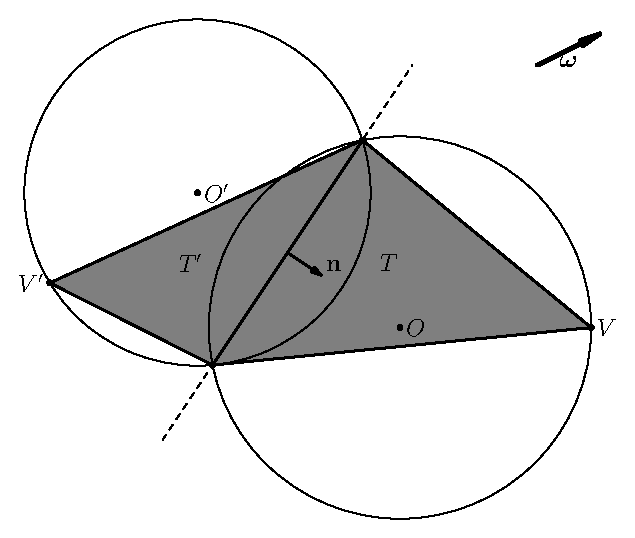
\includegraphics[height=.4\textheight]{spheres-0.eps}
\caption{К доказательству корректности упорядочения для триангуляций Делоне}
\label{fig:spheres}
\end{figure}
\[
V(T) = \frac{1}{3} S \vec n \overrightarrow{MV}, \qquad V(T') = \frac{1}{3} S \vec n \overrightarrow{V'M},
\]
где $S$ --- площадь их общей грани. Суммируя и учитывая $V(T) + V(T') > 0$, получаем
\[
\vec n \overrightarrow{V'V} > 0.
\]

Условие Делоне означает, что расстояние от точки $O$ до $V'$ должно быть больше расстояния от $O$ до $V$. Аналогично для второй сферы:
\[
|OV'| > |OV|, \quad |O'V| > |O'V'|.
\]
Возводя последние соотношения в квадрат, получаем
\[
(\overrightarrow{OV'},\overrightarrow{OV'}) - (\overrightarrow{OV},\overrightarrow{OV}) > 0, \qquad
(\overrightarrow{O'V},\overrightarrow{O'V}) - (\overrightarrow{O'V'},\overrightarrow{O'V'}) > 0
\]
Добавляя и вычитая $(\overrightarrow{OV'},\overrightarrow{OV})$, получаем
\begin{multline*}
0 < (\overrightarrow{OV'},\overrightarrow{OV'}) - (\overrightarrow{OV},\overrightarrow{OV}) =
(\overrightarrow{OV'},\overrightarrow{OV'}) 
-(\overrightarrow{OV'},\overrightarrow{OV})
+(\overrightarrow{OV'},\overrightarrow{OV})
- (\overrightarrow{OV},\overrightarrow{OV}) = \\ =
(\overrightarrow{OV'},\overrightarrow{VV'}) 
+
(\overrightarrow{VV'}, \overrightarrow{OV}) = 
\left(\overrightarrow{VV'}, \frac{\overrightarrow{OV}+ \overrightarrow{OV'}}{2}\right)
\end{multline*}
Аналогично,
\[
\left(\overrightarrow{V'V}, \frac{\overrightarrow{O'V}+ \overrightarrow{O'V'}}{2}\right)  =
\left(\overrightarrow{VV'}, \frac{\overrightarrow{VO'}+ \overrightarrow{V'O'}}{2}\right) 
> 0.
\]
Суммируя данные неравенства, получаем
\begin{equation}
(\overrightarrow{VV'},\overrightarrow{OO'}) > 0.
\label{eq:half}
\end{equation}
Так как точки $O,O'$ (а также $V,V'$) находятся в разных полупространствах, разделенных гранью, условие \eqref{eq:half} показывает, что точки $O$ и $V$ находятся с одной стороны грани, а $O'$ и $V'$ --- с другой. Таким образом, вектор $\overrightarrow{O'O}$ не только коллинеарен $\vec n$, но и сонаправлен с ним. Поэтому условие $T \succ T'$, эквивалентное $\vec \omega \vec n > 0$, эквивалентно $\vec \omega \overrightarrow{O'O} > 0$, что в свою очередь эквивалентно $\pi(T) > \pi(T')$. Полученное противоречие доказывает $T \prec T' \Rightarrow \pi(T) < \pi(T')$.

Используемые строгие неравенства предполагают общее расположение тетраэдров (описанные сферы двух тетраэдров не могут совпадать). Выполнения этого условия можно добиться небольшим возмущением триангуляции. Заметим, что для триангуляции Делоне невозможно образование циклов в отношении $\prec$.


\subsection{Алгоритм для триангуляций общего вида}

Для построения упорядочения $c(T)$ триангуляции общего вида можно воспользоваться модификацией алгоритма Тарьяна \cite{Corman2009} для топологической сортировки, который в свою очередь, является простой модификацией поиска в ширину.

В алгоритме \ref{alg:coloring} используется очередь тетраэдров, заполненная изначально тетраэдрами, у которых все входные грани освещены, то есть теми тетраэдрами, для которых на всех входных гранях задано граничное условие.

На очередном шаге алгоритма из очереди извлекается тетраэдр $T$. Проверяется, присвоен ли номер $c(T_j)$ всем его предшествующим соседям $T_j \prec T$. Если это так, тетраэдру $T$ присваивается номер
\[
c(T) = 1 + \max_{T_j \prec T} c(T_j).
\]
В случае, когда тетраэдр $T$ лежит на границе области, для отсутствующих соседей $T_j$ формально полагается $c(T_j) = 0$. Это позволяет присвоить всем тетраэдрам, которые изначально были в очереди номер $c(T) = 1$. После присвоения номера тетраэдру $T$, в очередь добавляются все следующие за ним тетраэдры $T' \succ T$, которым еще не присвоен номер.

Если хотя бы одному предшествующему соседу $T_j \prec T$ еще не присвоен номер, тетраэдр $T$ возвращается в конец очереди. Данный алгоритм способен определять наличие циклов в отношении $\prec$. Если в триангуляции обнаружен цикл, тетраэдры будут постоянно извлекаться и добавляться в конец очереди. Алгоритмически это можно определить используя счетчик. После добавления нового тетраэдра в очередь счетчик устанавливается равным длине очереди, а при возвращении тетраэдра обратно в очередь, счетчик уменьшается на единицу. Если на очередном шаге алгоритма счетчик обнуляется, это свидетельствует о том, что последние $n$ шагов алгоритма из очереди длины $n$ тетраэдры только извлекались и добавлялись обратно, причем ни одному новому тетраэдру не был присвоен номер. Данный факт свидетельствует о зацикливании алгоритма, а значит граф отношения $\prec$ не является ациклическим. Работа алгоритма проиллюстрирована на рисунке \ref{fig:coloring}.
\begin{figure}[ht!]
\centering
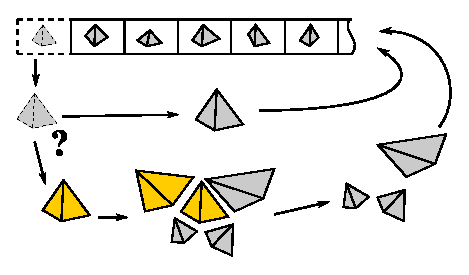
\includegraphics[height=.3\textheight]{coloring.eps}
\caption{Иллюстрация работы алгоритма упорядочения}
\label{fig:coloring}
\end{figure}

\begin{algorithm}[ht!]
\centering
\begin{algorithmic}[1]
\Procedure{Ordering}{}
\State $Q :=$ \Call{InitQueue}{}
\State $cnt := |Q|$
\While {$Q \neq \emptyset$}
\State $T :=$ \Call{Dequeue}{$Q$}
\If {$\forall T' \prec T, c(T') \neq \mathbf{nil}$}
\State $c(T) := 1 + \max_{T' \prec T} c(T')$
\For {$T'' \succ T: c(T'') = \mathbf{nil}$}
\State \Call{Enqueue}{$Q$, $T''$}
\EndFor
\State $cnt := |Q|$
\Else
\State \Call{Enqueue}{$Q$, $T$}
\State $cnt := cnt - 1$;
\EndIf
\If {$cnt < 0$}
\State \textbf{error} В триангуляции обнаружен цикл.
\EndIf
\EndWhile
\EndProcedure
\end{algorithmic}
\caption{Алгоритм упорядочения для произвольной триангуляции}
\label{alg:coloring}
\end{algorithm}

Заметим, что данное упорядочение является оптимальным в том смысле, что каждому тетраэдру $T$ присваивается минимально возможный номер $c(T)$. При этом максимальный номер будет присвоен последнему тетраэдру в самой длинной цепочке зависимых тетраэдров
\[
T_1 \prec T_2 \prec \dots \prec T_n.
\]

\section{Связь минимального порядка $c(T)$ с ярусно-параллельной формой алгоритма}

Если упорядочение $c(T)$ минимально, например, построено с помощью алгоритма \ref{alg:coloring}, то множество всех тетраэдров сетки разбивается на непересекающиеся подмножества
\[
U_k = \left\{T \mid c(T) = k\right\}.
\]
При этом для вычисления решения в каждом тетраэдре $T \in U_k$ достаточно знать решения для каждого тетраэдра $T' \in \bigcup_{j = 1}^{k - 1} U_j$. В частности, решение в $T$ не зависит от решения в тетраэдрах $T''$ с тем же номером $c(T'') = k$. Последнее свойство означает, что решения во всех тетраэдрах из $U_k$ можно находить параллельно.

Заметим, что ациклический граф отношения $\prec$ является также графом зависимостей вычислительного алгоритма, а построенное упорядочение фактически задает ярусно-параллельную его форму \cite{Karpov2014}. По определению, ярусно-параллельной формой называется деление графа на такие множества $V_i$, что для каждой дуги $u \to v, u \in V_j, v \in V_k$ выполняется $j < k$.
В маршевом методе решение вычисляется последовательно для каждого множества $U_k, k = 1, \dots, n$, но в каждом множестве $U_k$ решение может вычисляться параллельно. На рисунке \ref{fig:marching} показаны тетраэдры, в которых решение уже вычислено для различных моментов <<марша>>: в начале, в середине и в конце.

\begin{figure}[ht!]
\centering
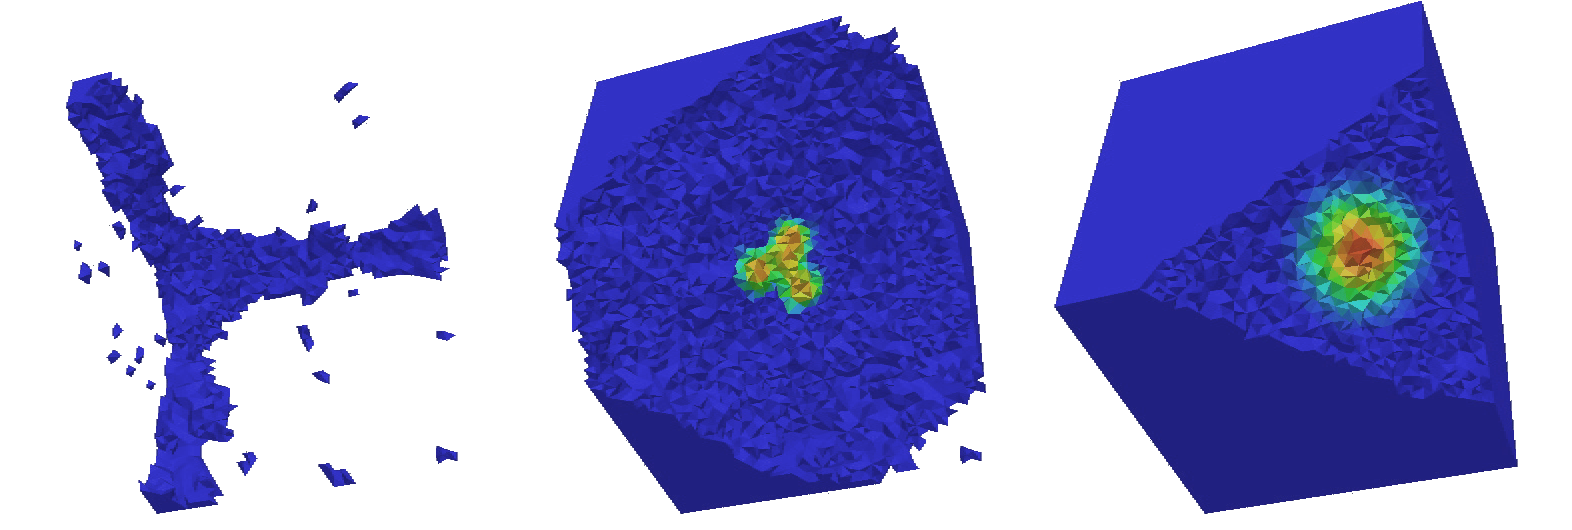
\includegraphics[height=.2\textheight]{123.png}
\caption{Множество тетраэдров с номером $c(T) < k$ для различных $k$}
\label{fig:marching}
\end{figure}

Однако, для параллельной реализации алгоритма требуется учитывать накладные расходы на построение упорядочения $c(T)$. Алгоритм упорядочения существенно последователен, поэтому выигрыш от распараллеливания возможен лишь в двух случаях
\begin{itemize}
\item решение задачи в каждом тетраэдре ресурсоемко, например, одновременно решается уравнение переноса для большого числа частот;
\item производится многократное решение уравнения переноса, например, на протяжении большого числа шагов по времени.
\end{itemize}
В последнем случае для каждого направления переноса необходимо хранить упорядочение $c(T)$. К тому же, между шагами по времени не должна изменяться расчетная сетка. Последнее обстоятельство сильно ограничивает применимость параллельного алгоритма на подвижных сетках.